\title[\LaTeX\ and Web]{Madagascar \\
\LaTeX\ and Web tools}

\author[S. Fomel] % (optional, nur bei vielen Autoren)
{Sergey~Fomel}
% - Der \inst{?} Befehl sollte nur verwendet werden, wenn die Autoren
%   unterschiedlichen Instituten angeh�ren.

\institute[UT Austin] % (optional, aber oft n�tig)
{
  Bureau of Economic Geology \\
  Jackson School of Geosciences \\
  University of Texas at Austin
}

\date[Vancouver School \& Workshop]{August 30, 2006}

\begin{frame}
  \titlepage
\end{frame}

\begin{frame}
  \frametitle{The Big Scheme of Things}
  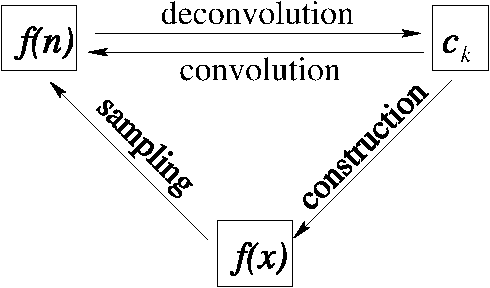
\includegraphics[height=0.8\textheight]{XFig/Fig/scheme}
\end{frame}

\begin{frame}
  \frametitle{The Big Scheme of Things II}
  \includegraphics[height=0.8\textheight]{XFig/Fig/scheme2}
\end{frame}

\begin{frame}
  \frametitle{Outline}
  \tableofcontents[pausesections]
\end{frame}

\section{\LaTeX\ tools}
\begin{frame}<beamer>
  \frametitle{Outline}
  \tableofcontents[currentsection]
\end{frame}

\begin{frame}
  \frametitle{SEGTeX package}
  \begin{itemize}
  \item Started in June 2003
  \item 6 main contributors
  \item Version 0.9 released June 2006
  \item Development version
    \begin{itemize}
    \item 2,000 revisions
    \item 300 main programs (140,000 lines of C) 
    \item 3,000 tests (40,000 lines of Python)
    \item 30 papers (20,000 lines of \LaTeX)
    \end{itemize}
  \item \url{http://rsf.sf.net/}
  \end{itemize}
\end{frame}

\begin{frame}
  \frametitle{Heritage}
  \begin{itemize}
  \item SEPlib
    \begin{itemize}
    \item Rob Clayton, Jon
      Claerbout, Dave Hale, Stew Levin, Rick Ottolini, Joe Dellinger, Steve
      Cole, Dave Nichols, Martin Karrenbach, Biondo Biondi, Bob Clapp
    \end{itemize}
  \item SEP reproducible research system
    \begin{itemize}
    \item  Martin Karrenbach, Matthias Schwab, Joel Schroeder, Sergey Fomel, 
    Bob Clapp
    \end{itemize}
  \item Seismic Unix
  \item DDS
  \end{itemize}
\end{frame}

\section{From \LaTeX\ to PDF}
\begin{frame}<beamer>
  \frametitle{Outline}
  \tableofcontents[currentsection]
\end{frame}

\begin{frame}
  \frametitle{Test Driven Development}
  \begin{itemize}
  \item XP, agile software engineering, refactoring
    \begin{itemize}
    \item Tests drive development
    \end{itemize}
  \item Computational geophysics
    \begin{itemize}
    \item Tests are numerical experiments
    \end{itemize}
  \item Science
    \begin{itemize}
      \item Reproducible experiments mean \href{http://egl.beg.utexas.edu/RSF/}{progress}
    \end{itemize}
  \end{itemize}
\end{frame}

\begin{frame}
\frametitle{Reproducible Research Tools}
\begin{itemize}
\item SEP
\begin{itemize}
\item GNU make rules
\item Perl scripts
\item Shell scripts
\item \LaTeX\ macros
\end{itemize}
\item Madagascar
\begin{itemize}
\item SCons (Python replacement for make)
\end{itemize}
\end{itemize}
\end{frame}

\section{From \LaTeX\ to HTML}
\begin{frame}<beamer>
  \frametitle{Outline}
  \tableofcontents[currentsection]
\end{frame}

\begin{frame}
  \frametitle{Open Source}
  \begin{itemize}
  \item Open source means freedom to the user
    \begin{itemize}
    \item Freedom to use
	\item Freedom to study and modify
	\item Freedom to redistribute 
	\item Freedom to improve 
    \end{itemize}
  \item Open source means collaboration and peer review
  \item Madagascar package is 100\% open-source
    \begin{itemize}
      \item GPL license
      \item Hosted by Sourceforge
      \item Developed with Subversion
    \end{itemize}
  \end{itemize}
\end{frame}

\section{Dynamic Web Services}
\begin{frame}<beamer>
  \frametitle{Outline}
  \tableofcontents[currentsection]
\end{frame}

\begin{frame}
  \frametitle{Communication Tools}
  \begin{itemize}
  \item Mailing Lists
  \item Forums
  \item Blog and RSS
  \item Wiki
  \end{itemize}
\end{frame}

\section*{Lessons}

\begin{frame}
  \frametitle{Summary}
  \begin{itemize}
  \item Madagascar is a software package for geophysical data processing and
    reproducible numerical experiments.
  \item New, test-driven, open-source, using a universal file format
  \end{itemize}
\end{frame}

\begin{frame}
  \frametitle{Please Visit}
  \begin{itemize}
  \item {\Huge \color{yellow}{\url{http://rsf.sf.net}}}
  \item School and workshop 
    \begin{itemize}
    \item \emph{Reproducible Research in Computational Geophysics}
    \item August 30-31, 2006
    \item Vancouver BC, Canada
    \end{itemize}
  \end{itemize}
\end{frame}

